\begin{fact} \label{quadri}
	Considérons tous les quadrilatères de périmètre fixé $p$. Parmi tous ces quadrilatères, un seul est d'aire maximale, c'est le carré de côté $c = \num{.25} p$.
\end{fact}


\begin{proof}
	Rappelons, ou indiquons, qu'un quadrilatère $\setproba{Q}$ est convexe si pour toute paire de points $M$ et $N$ de la surface associée à $\setproba{Q}$, le segment $[MN]$ est contenu dans cette surface (cette définition se généralise aux polygones).
	La figure suivante montre que pour tout quadrilatère $ABCD$ non convexe en $B$, et de périmètre $p$, il existe un quadrilatère convexe $AB^{\,\prime}CD$ de périmètre $p$, et tel que $\area{AB^{\,\prime}CD} > \area{ABCD}$.
	Notre recherche doit donc continuer dans l'ensemble des quadrilatères convexes de périmètre $p$.

	\begin{center}
		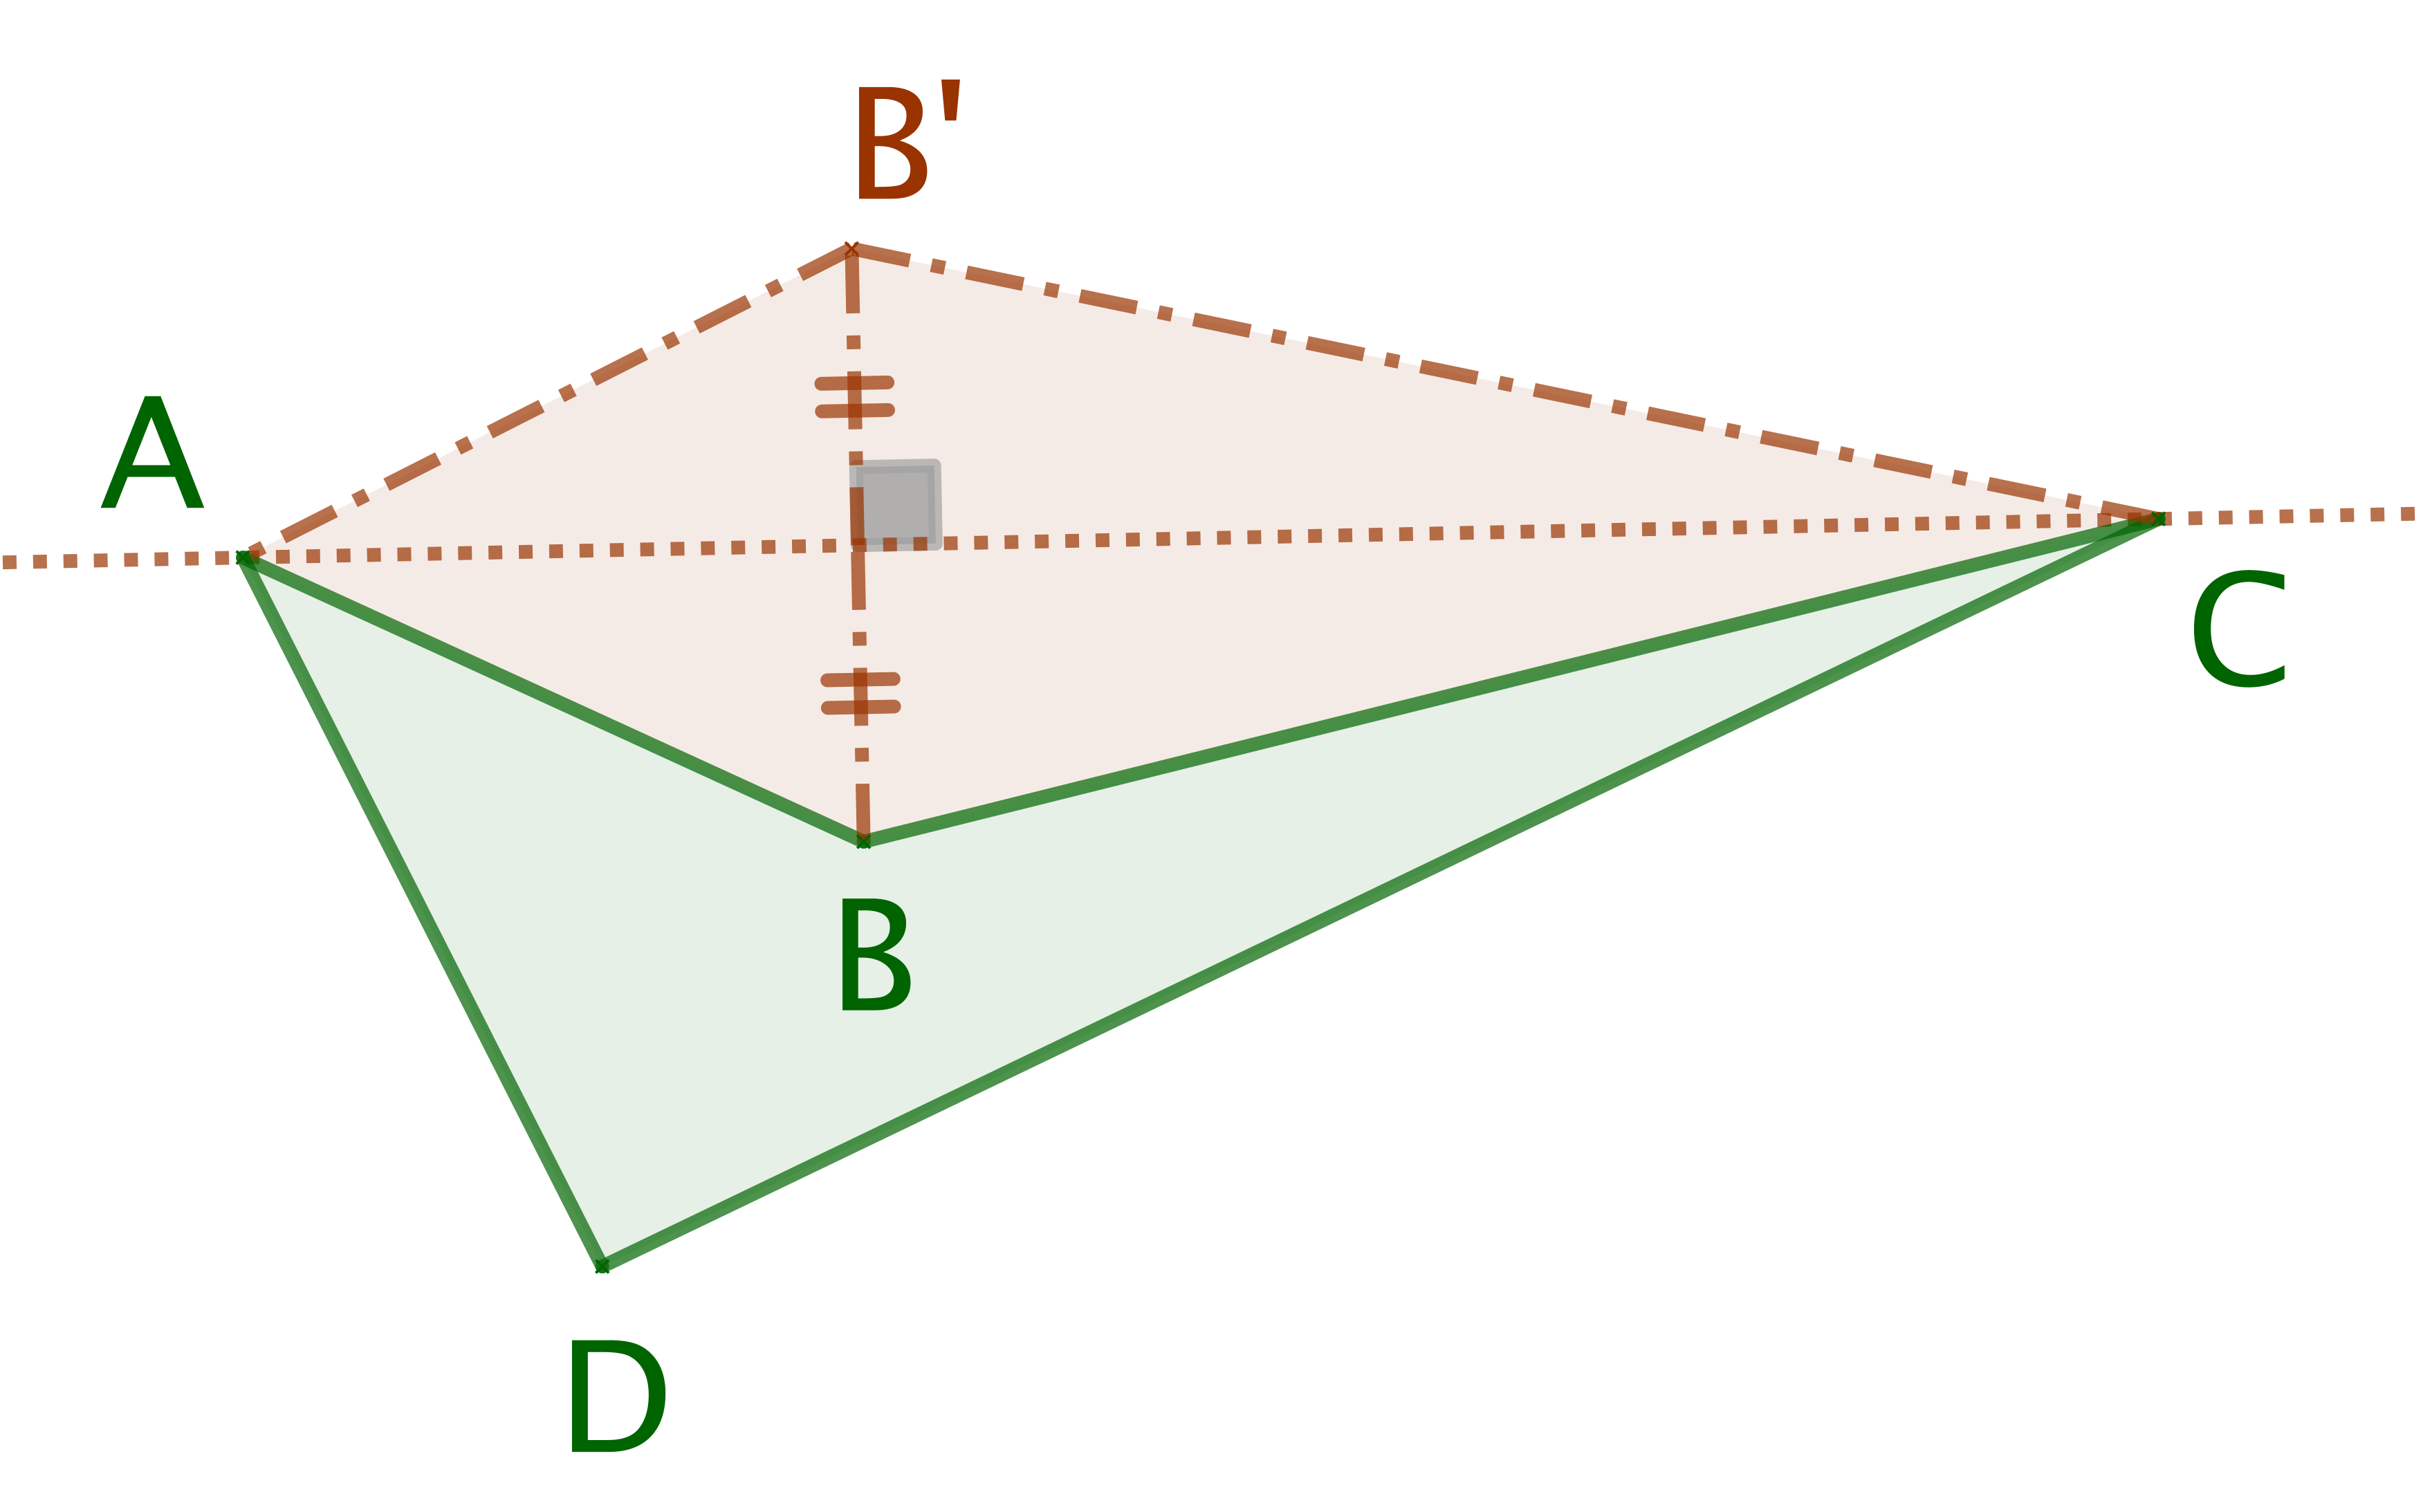
\includegraphics[scale=.4]{content/quadrilateral/non-convex.png}
	\end{center}
	
	
	Si un quadrilatère convexe $ABCD$ de périmètre $p$ est tel que $AB \neq BC$, le fait \ref{tri-one-side-fixed} nous donne un quadrilatère convexe $AB^{\,\prime}CD$ de périmètre $p$,%
	\footnote{
		Noter que
		$\perim{AB^{\,\prime}CD} = \perim{AB^{\,\prime}C} + \perim{ACD} - 2 AC$.
	}
	et vérifiant aussi $AB^{\,\prime} = B^{\,\prime}C$ et $\area{AB^{\,\prime}CD} > \area{ABCD}$ comme le montre la figure ci-après.
	On se ramène donc au cas d'un quadrilatère convexe $ABCD$ de périmètre $p$ avec en plus $AB = BC$.

	\begin{center}
		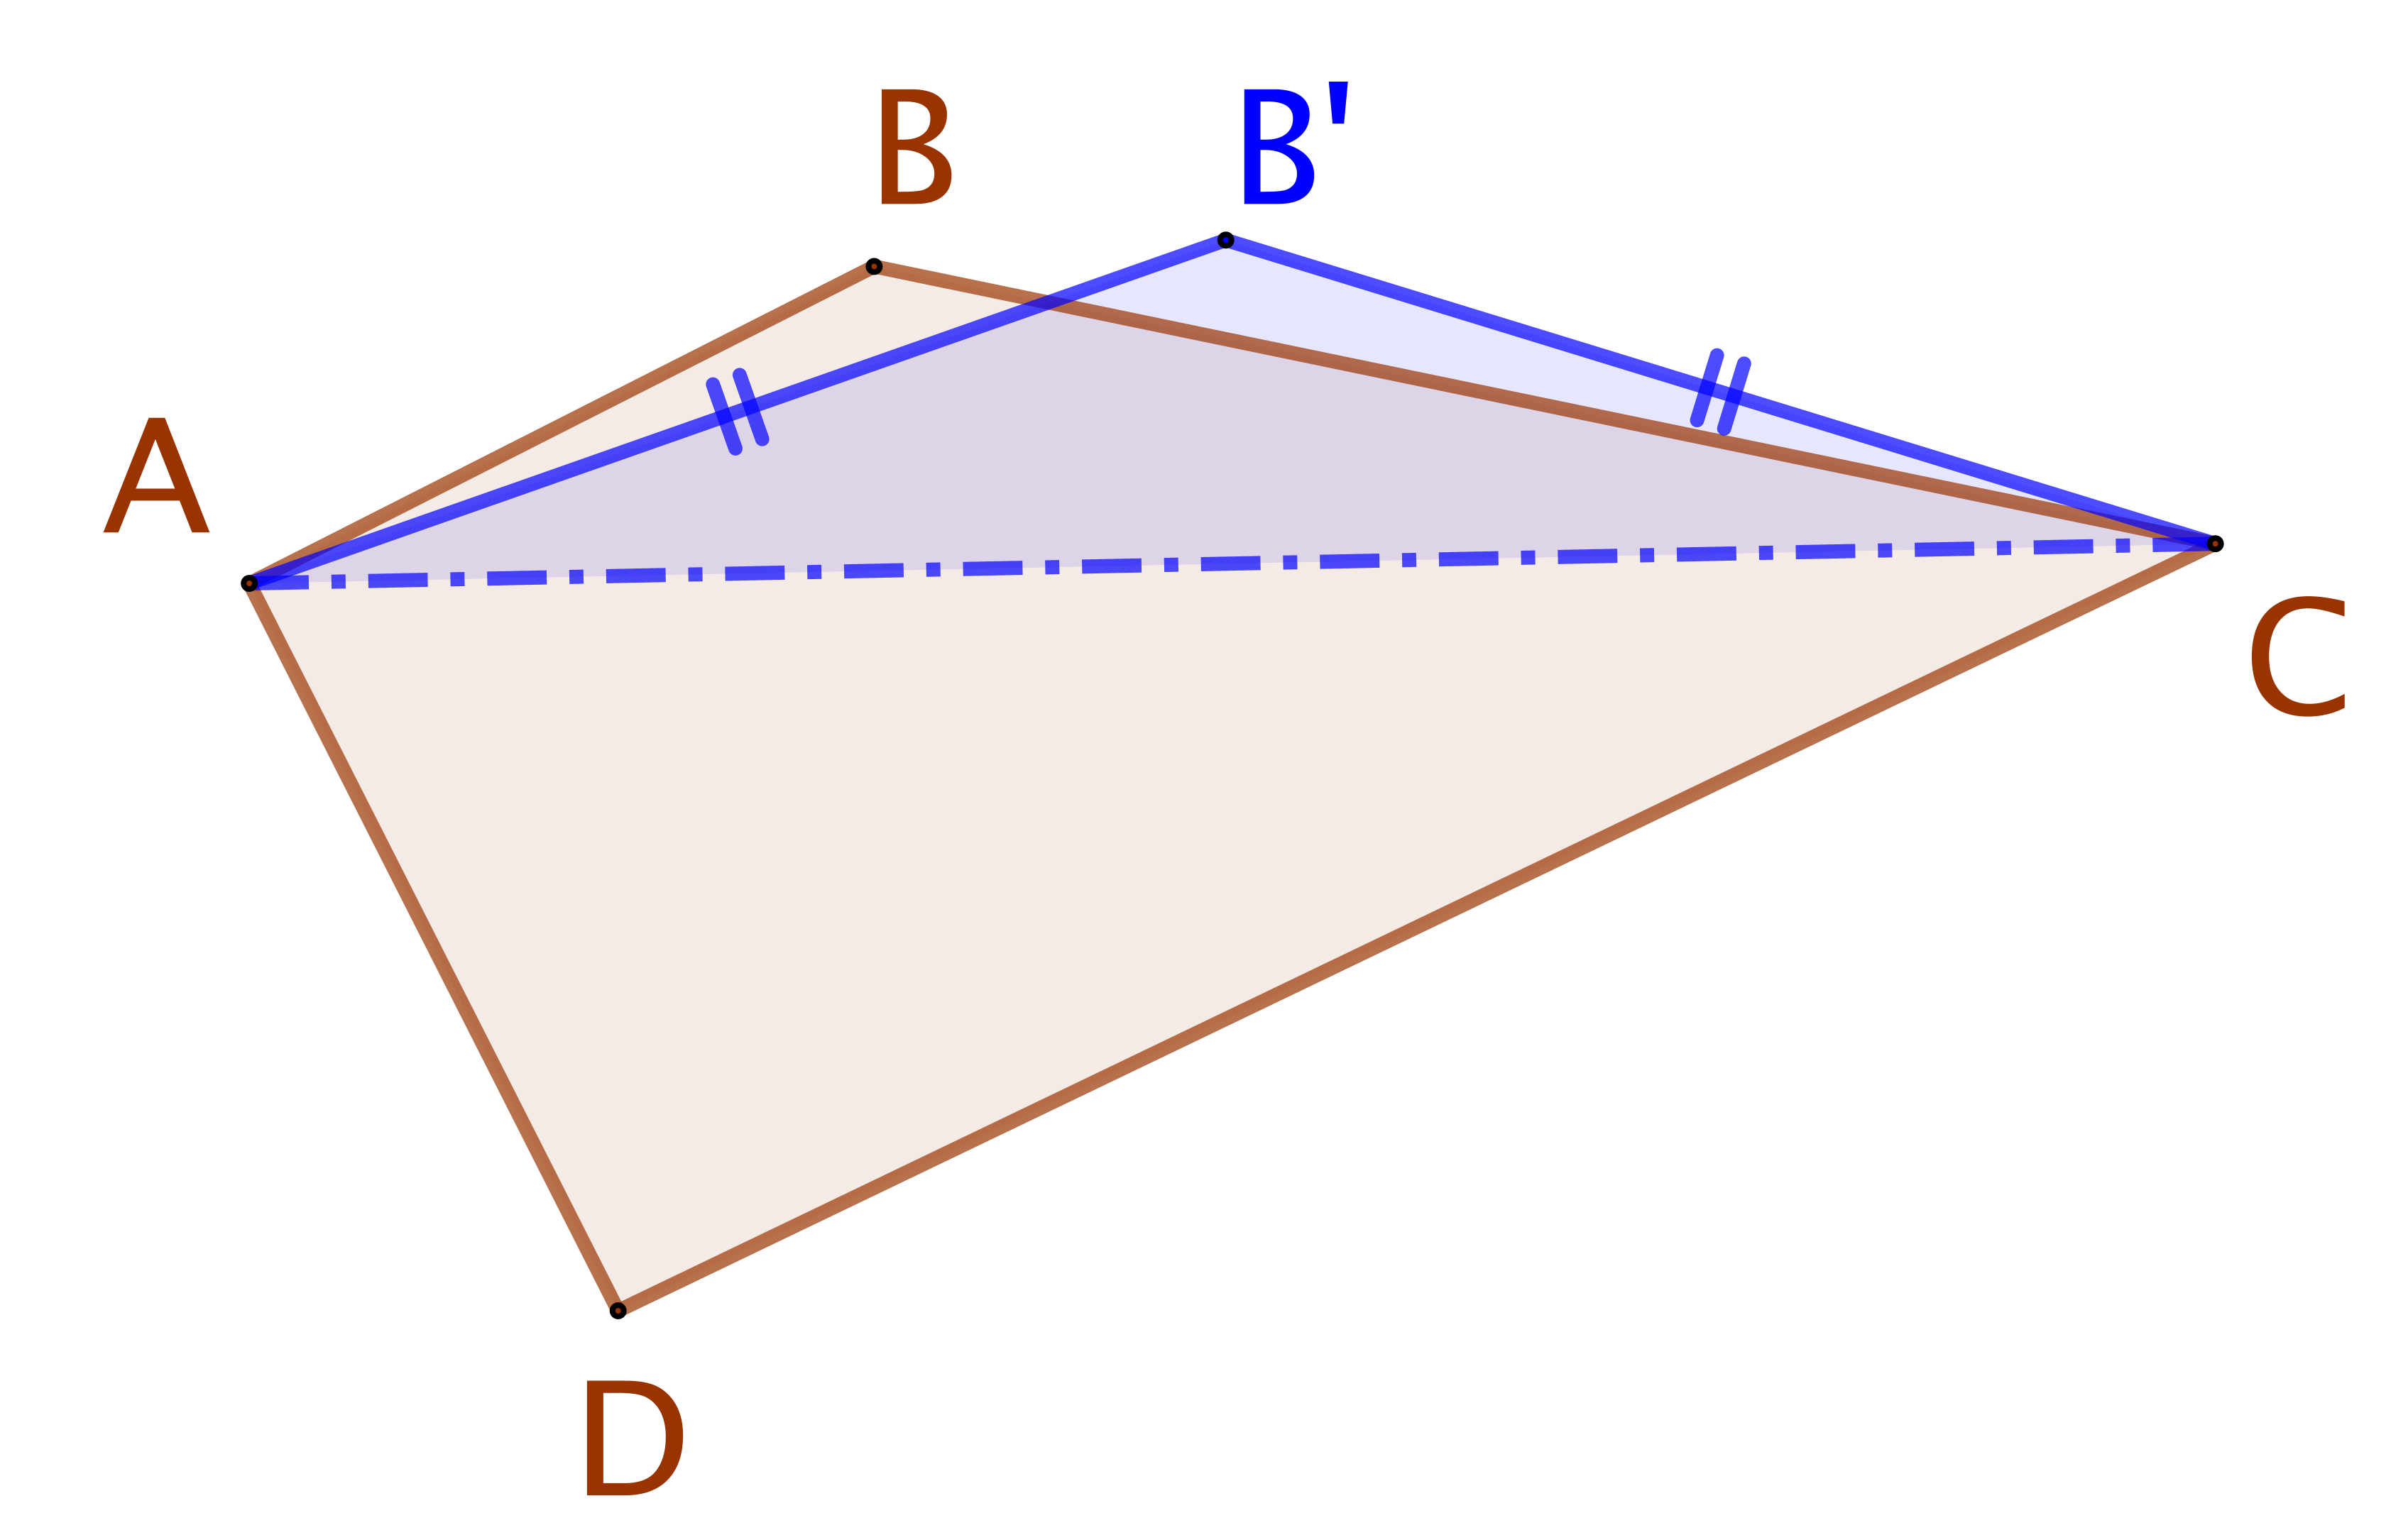
\includegraphics[scale=.4]{content/quadrilateral/convex-gene.png}
	\end{center}
	
	
	La méthode précédente appliquée au sommet $D$ d'un quadrilatère convexe $ABCD$ de périmètre $p$ tel que $AB = BC$ et $AD \neq DC$ permet en fait de se ramener au cas d'un cerf-volant $ABCD$ de périmètre $p$, avec $AB = BC$ et $AD = DC$, voir ci-dessous. 

	\begin{center}
		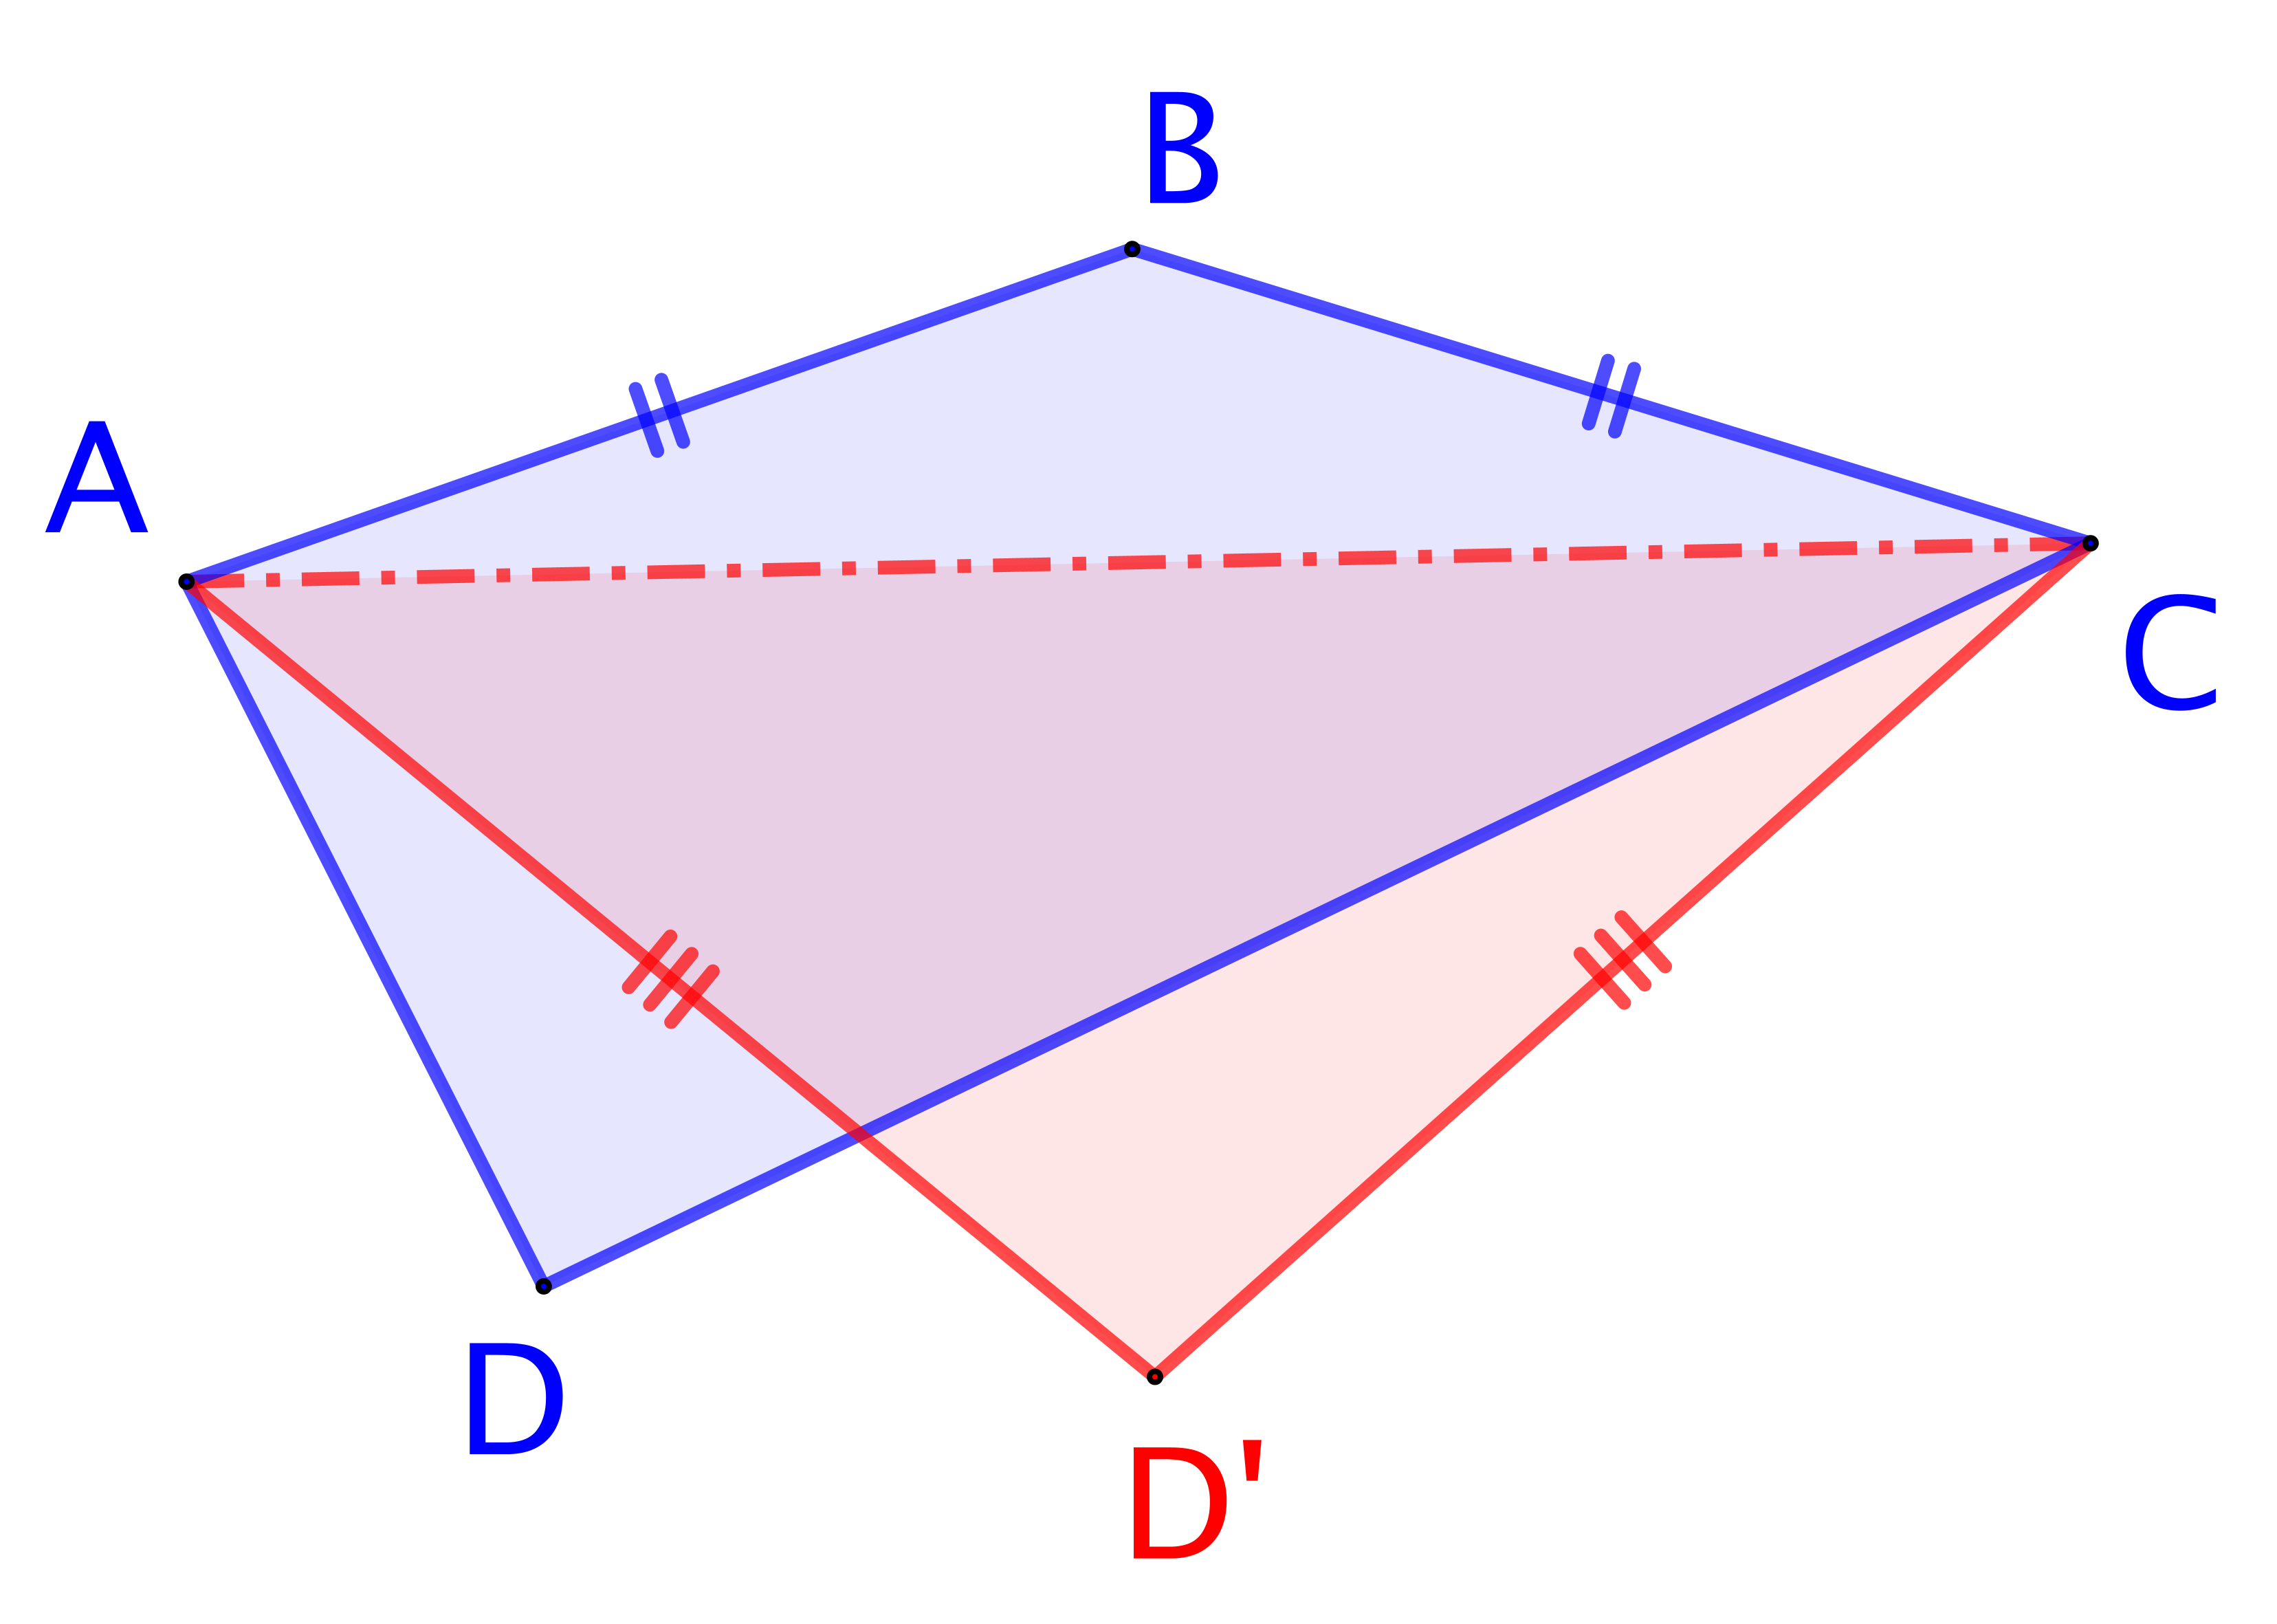
\includegraphics[scale=.4]{content/quadrilateral/convex-one-paire.png}
	\end{center}
	
	
	En supposant que notre cerf-volant ne soit pas un losange, le fait \ref{tri-one-side-fixed} appliqué aux sommets $A$ et $C$ fournit un losange $A^{\,\prime}BC^{\,\prime}D$ de périmètre $p$, et tel que $\area{A^{\,\prime}BC^{\,\prime}D} > \area{ABCD}$.
	%
	En effet, nous avons
	$p = 2(AB + AD)$
	et
	$\perim{A^{\,\prime}BD} = \perim{ABD}$,
	donc
	$A^{\,\prime}B = A^{\,\prime}D = \num{.25} p$,
	et de même, nous obtenons
	$C^{\,\prime}B = C^{\,\prime}D = \num{.25} p$.

	\begin{center}
		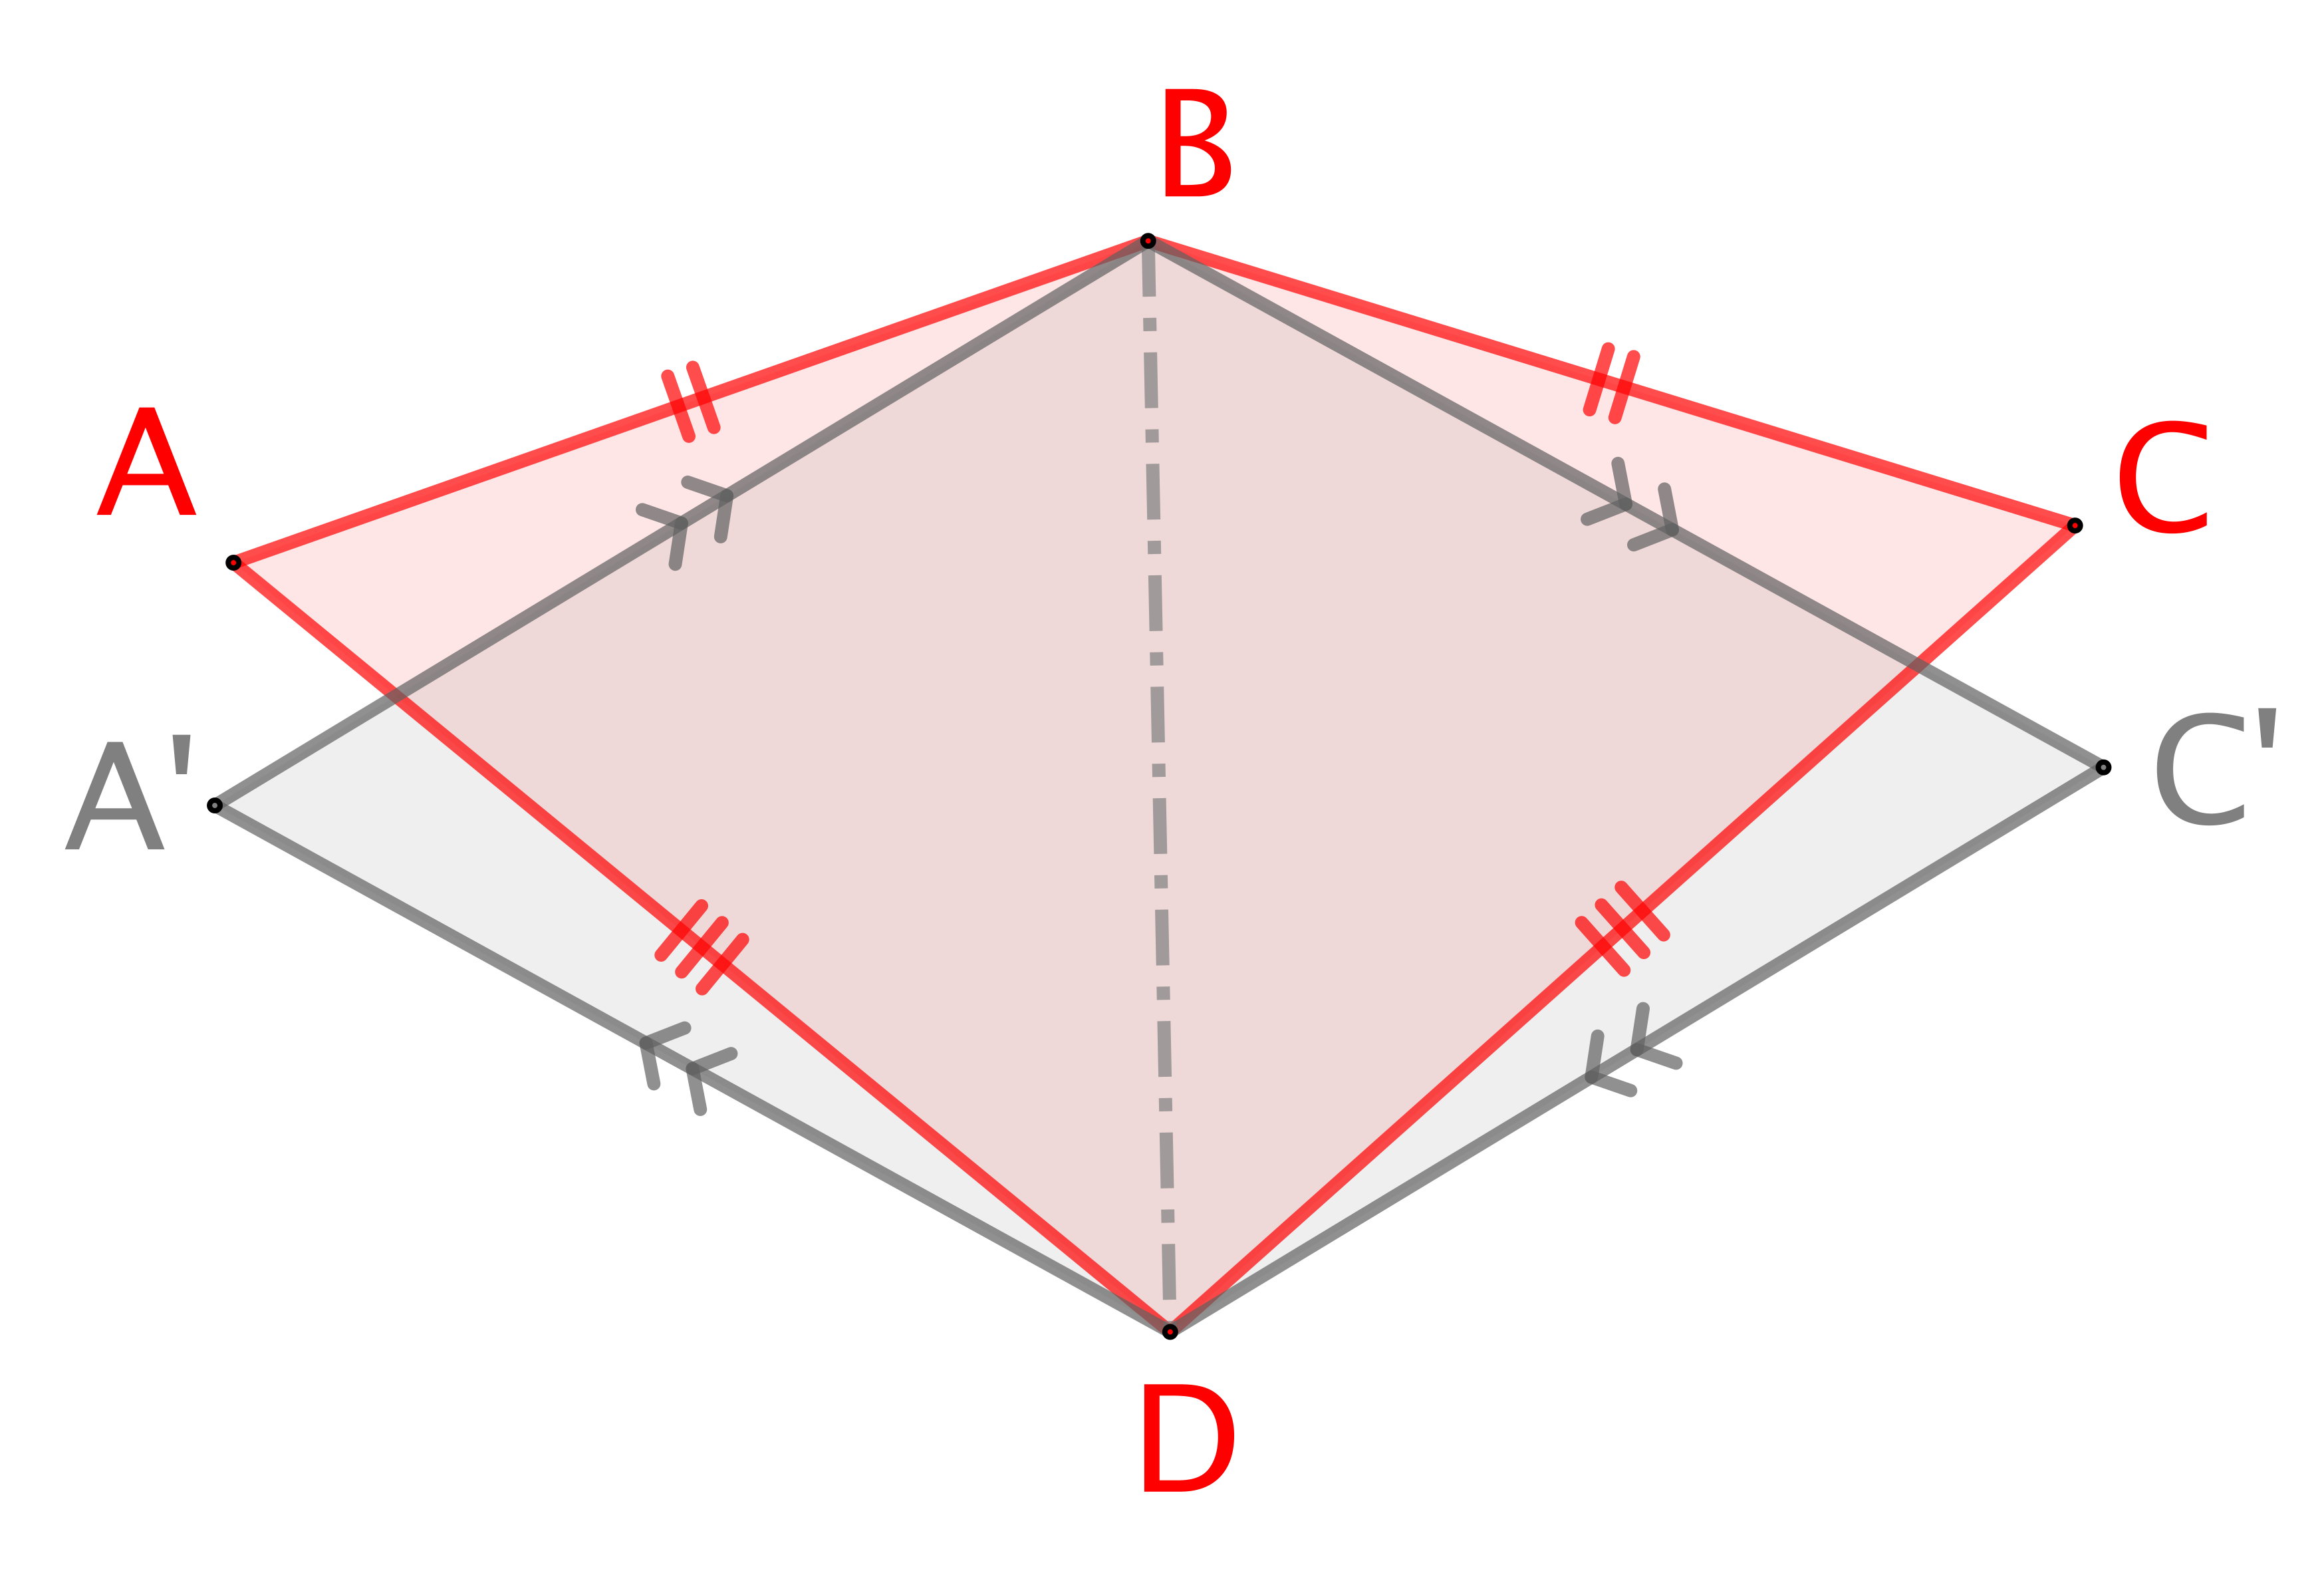
\includegraphics[scale=.4]{content/quadrilateral/convex-isopaire.png}
	\end{center}
	
	
	Pour conclure, il suffit d'appliquer le fait \ref{iso-para}, puisque tout losange est un parallélogramme. Que la géométrie est belle!
\end{proof}
